\documentclass[aspectratio=169]{beamer}
\usetheme{A}


% -- packages
\usepackage{transparent}
\usepackage{fontspec}
\usepackage{libertinus-otf}
\usepackage{etoolbox}
\usepackage{enumitem}
\usepackage{graphicx}
\usepackage{emoji}
\usepackage{relsize}
\usepackage{hyperref}
\hypersetup{
    colorlinks=true,
    linkcolor=blue,  % Change link color to blue
    urlcolor=blue    % Change URL color to blue
}
\usepackage{booktabs}
\usepackage{tikz}
\usepackage{pgfplots}
\usetikzlibrary{decorations.pathmorphing,calc,fit,scopes,shapes,positioning}
\usepackage{tikz-qtree}
\usepackage{amsmath}
\usepackage{proof}
\usepackage{adjustbox}
\usepackage{eqparbox}
\usepackage{soul}
\usepackage{tabularx}
\usepackage{emoji}

% -- options 
\setbeamercovered{transparent=20}
\setlist[itemize]{label=\textcolor{pred}{$\bullet$}, topsep=0pt, itemsep=0pt}
\setlist[itemize,2]{label=\textcolor{pred}{$\circ$}, topsep=0pt, itemsep=0pt,leftmargin=1.5em}

\newcommand{\light}[1]{\textcolor{light}{#1}}
\definecolor{light}{rgb}{0.35,0.35,0.35}
\definecolor{red}{HTML}{D20000}
\definecolor{blue}{HTML}{0000CD}
\definecolor{green}{HTML}{007100}
\newcounter{tokencounter}
\newcommand{\token}[1]{%
  \stepcounter{tokencounter}%
  \pgfmathsetmacro{\opacity}{1 - \thetokencounter / 180}%
  \ifdim \opacity pt < 0pt
    \def\opacity{0}
  \fi
  \transparent{\opacity}{\fcolorbox{gray}{white}{\textcolor{black!70}{\strut{\detokenize{#1}}}}}%
}
\newcounter{remarkcounter}
\newcommand{\remark}[1]{%
%	\light{\textbf{Remark \theremarkcounter{}.} #1}%
	\begin{flushright}
	#1	
	\end{flushright}
	\stepcounter{remarkcounter}%
}
\newcommand{\overlaytext}[3]{%
  \tikz[remember picture, overlay]{%
    \node[anchor=base] at (#1,#2) {#3};%
  }%
}
\newcommand{\hole}[2]{\alt<{#1}>{\AgdaHole{\smaller ?}}{#2}}
\newcommand{\stdlib}{\texttt{stdlib}}
\newcommand\unimath{\texttt{Unimath}}
\newcommand\typetopo{\texttt{TypeTopo}}
\newcommand\agdaQuill{\textsc{Quill}}	


\title{Towards Structure-Aware Neural Representations\\
 of Agda Programs}
\date{%
	\vspace{-2em}\\
		Theorem Proving and Machine Learning in the age of LLMs\\
		April 2025, Edinburgh
		
	\vspace{4em}
	\smaller
	\begin{flushleft}
	\light{
	\eqmakebox[bla][l]{Publication} : Learning Structure-Aware Representations of Dependent Types @ \textbf{NeurIPS} 2024\\
	\eqmakebox[bla][l]{ACK} : Funds from \textbf{EuroProofNet CA2011} (2 STSMs in 2023)
	}	
	\end{flushleft}
}
\author{\light{Konstantinos Kogkalidis, Orestis Melkonian, Jean-Philippe Bernardy}}

\newcommand{\agdafont}{\scriptsize}
\newcommand{\sstat}[2]{\hphantom{1}\ensuremath{#1}}
\newcommand{\bstat}[2]{\ensuremath{#1}}
\newcommand{\bfstat}[2]{\ensuremath{\mathbf{#1}}}
%%%%%%%%%%
% Minted %
%%%%%%%%%%
\usepackage{minted}

%%%%%%%%
% Agda %
%%%%%%%%
\usepackage[conor]{agda}
\AtBeginEnvironment{code}{\agdafont}
\usepackage{newunicodechar}
\newunicodechar{ℕ}{\ensuremath{\mathbb{N}}}
\newunicodechar{λ}{\ensuremath{\mathnormal\lambda}}
\newunicodechar{→}{\ensuremath{\mathnormal\to}}
\newunicodechar{∀}{\ensuremath{\mathnormal\forall}}
\newunicodechar{≡}{\ensuremath{\mathnormal\equiv}}
\newunicodechar{⋯}{\ensuremath{\mathnormal\dots}}
\newcommand\AD[1]{\AgdaDatatype{\agdaFontSize#1}}
\newcommand\AF[1]{\AgdaFunction{\agdaFontSize#1}}
\newcommand\AS[1]{\AgdaSymbol{\agdaFontSize#1}}
\newcommand\AB[1]{\AgdaBound{\agdaFontSize#1}}
\newcommand\AK[1]{\AgdaKeyword{\agdaFontSize#1}}
\usepackage{lipsum}

\begin{document}


\maketitle

\begin{frame}{\st{Mandatory (?)} Redundant Intro Slide}
	\smaller
	\textbf{Automated Theorem Proving}\\
	\light{\lipsum[1][1-2]}\\

	\textbf{Automated Theorem Proving in the Times of ML}\\
	\light{\lipsum[1][3-5]}
\end{frame}

\begin{frame}[fragile, plain]{\alt<2->{... what Agda shows you}{Proving stuff (in Agda): what you write}}
	\smaller
	\only<1>{		
	    % Aspect colours.
	    \definecolor{AgdaComment}      {HTML}{000000}
	    \definecolor{AgdaPragma}       {HTML}{000000}
	    \definecolor{AgdaKeyword}      {HTML}{000000}
	    \definecolor{AgdaString}       {HTML}{000000}
	    \definecolor{AgdaNumber}       {HTML}{000000}
	    \definecolor{AgdaSymbol}       {HTML}{000000}
	    \definecolor{AgdaPrimitiveType}{HTML}{000000}
	
	    % NameKind colours.
	    \definecolor{AgdaBound}                 {HTML}{000000}
	    \definecolor{AgdaGeneralizable}         {HTML}{000000}
	    \definecolor{AgdaInductiveConstructor}  {HTML}{000000}
	    \definecolor{AgdaCoinductiveConstructor}{HTML}{000000}
	    \definecolor{AgdaDatatype}              {HTML}{000000}
	    \definecolor{AgdaField}                 {HTML}{000000}
	    \definecolor{AgdaFunction}              {HTML}{000000}
	    \definecolor{AgdaMacro}                 {HTML}{000000}
	    \definecolor{AgdaModule}                {HTML}{000000}
	    \definecolor{AgdaPostulate}             {HTML}{000000}
	    \definecolor{AgdaPrimitive}             {HTML}{000000}
	    \definecolor{AgdaRecord}                {HTML}{000000}
	    \definecolor{AgdaArgument}              {HTML}{000000}
	
	    % Other aspect colours.
	    \definecolor{AgdaDottedPattern}     {HTML}{000000}
	    \definecolor{AgdaUnsolvedMeta}      {HTML}{D3D3D3}
	    \definecolor{AgdaUnsolvedConstraint}{HTML}{D3D3D3}
	    \definecolor{AgdaTerminationProblem}{HTML}{BEBEBE}
	    \definecolor{AgdaIncompletePattern} {HTML}{D3D3D3}
	    \definecolor{AgdaErrorWarning}      {HTML}{BEBEBE}
	    \definecolor{AgdaError}             {HTML}{696969}
	
	    % Misc.
	    \definecolor{AgdaHole}              {HTML}{BEBEBE}
	}
	\begin{minipage}{0.9\textwidth}
	\begin{code}%
	\>[0]\AgdaKeyword{open}\AgdaSpace{}%
	\AgdaKeyword{import}\AgdaSpace{}%
	\AgdaModule{Relation.Binary.PropositionalEquality}\AgdaSpace{}%
	\AgdaKeyword{using}\AgdaSpace{}%
	\AgdaSymbol{(}\AgdaOperator{\AgdaDatatype{\AgdaUnderscore{}≡\AgdaUnderscore{}}}\AgdaSymbol{;}\AgdaSpace{}%
	\AgdaInductiveConstructor{refl}\AgdaSymbol{;}\AgdaSpace{}%
	\AgdaFunction{cong}\AgdaSymbol{;}\AgdaSpace{}%
	\AgdaFunction{trans}\AgdaSymbol{)}\<%
	\end{code}
	
	\vspace{-1.25em}
	\begin{minipage}{.3\linewidth}
	\begin{code}%
	\>[0]\AgdaKeyword{data}\AgdaSpace{}%
	\AgdaDatatype{ℕ}\AgdaSpace{}%
	\AgdaSymbol{:}\AgdaSpace{}%
	\AgdaPrimitive{Set}\AgdaSpace{}%
	\AgdaKeyword{where}\<%
	\\
	\>[0][@{}l@{\AgdaIndent{0}}]%
	\>[2]\AgdaInductiveConstructor{zero}%
	\>[8]\AgdaSymbol{:}\AgdaSpace{}%
	\AgdaDatatype{ℕ}\<%
	\\
	%
	\>[2]\AgdaInductiveConstructor{suc}%
	\>[8]\AgdaSymbol{:}\AgdaSpace{}%
	\AgdaDatatype{ℕ}\AgdaSpace{}%
	\AgdaSymbol{→}\AgdaSpace{}%
	\AgdaDatatype{ℕ}\<%
	\end{code}
	\end{minipage}
	
	\vspace{-1.25em}
	\begin{minipage}{.5\linewidth}
	\begin{code}%
	\>[0]\AgdaOperator{\AgdaFunction{\AgdaUnderscore{}+\AgdaUnderscore{}}}\AgdaSpace{}%
	\AgdaSymbol{:}\AgdaSpace{}%
	\AgdaDatatype{ℕ}\AgdaSpace{}%
	\AgdaSymbol{→}\AgdaSpace{}%
	\AgdaDatatype{ℕ}\AgdaSpace{}%
	\AgdaSymbol{→}\AgdaSpace{}%
	\AgdaDatatype{ℕ}\<%
	\\
	\>[0]\AgdaInductiveConstructor{zero}%
	\>[7]\AgdaOperator{\AgdaFunction{+}}\AgdaSpace{}%
	\AgdaBound{n}\AgdaSpace{}%
	\AgdaSymbol{=}\AgdaSpace{}%
	\AgdaBound{n}\<%
	\\
	\>[0]\AgdaInductiveConstructor{suc}\AgdaSpace{}%
	\AgdaBound{m}%
	\>[7]\AgdaOperator{\AgdaFunction{+}}\AgdaSpace{}%
	\AgdaBound{n}\AgdaSpace{}%
	\AgdaSymbol{=}\AgdaSpace{}%
	\AgdaInductiveConstructor{suc}\AgdaSpace{}%
	\AgdaSymbol{(}\AgdaBound{m}\AgdaSpace{}%
	\AgdaOperator{\AgdaFunction{+}}\AgdaSpace{}%
	\AgdaBound{n}\AgdaSymbol{)}\<%
	\end{code}
	\end{minipage}
	
	\vspace{-1.25em}
	\begin{code}%
	\>[0]\AgdaFunction{+-comm}\AgdaSpace{}%
	\AgdaSymbol{:}\AgdaSpace{}%
	\AgdaSymbol{(}\AgdaBound{m}\AgdaSpace{}%
	\AgdaBound{n}\AgdaSpace{}%
	\AgdaSymbol{:}\AgdaSpace{}%
	\AgdaDatatype{ℕ}\AgdaSymbol{)}\AgdaSpace{}%
	\AgdaSymbol{→}\AgdaSpace{}%
	\AgdaBound{m}\AgdaSpace{}%
	\AgdaOperator{\AgdaFunction{+}}\AgdaSpace{}%
	\AgdaBound{n}\AgdaSpace{}%
	\AgdaOperator{\AgdaDatatype{≡}}\AgdaSpace{}%
	\AgdaBound{n}\AgdaSpace{}%
	\AgdaOperator{\AgdaFunction{+}}\AgdaSpace{}%
	\AgdaBound{m}\<%
	\\
	\>[0]\AgdaFunction{+-comm}\AgdaSpace{}%
	\AgdaInductiveConstructor{zero}%
	\>[16]\AgdaInductiveConstructor{zero}%
	\>[25]\AgdaSymbol{=}\AgdaSpace{}%
	\AgdaInductiveConstructor{refl}\<%
	\\
	\>[0]\AgdaFunction{+-comm}\AgdaSpace{}%
	\AgdaInductiveConstructor{zero}%
	\>[16]\AgdaSymbol{(}\AgdaInductiveConstructor{suc}\AgdaSpace{}%
	\AgdaBound{n}\AgdaSymbol{)}%
	\>[25]\AgdaSymbol{=}\AgdaSpace{}%
	\AgdaFunction{cong}\AgdaSpace{}%
	\AgdaInductiveConstructor{suc}\AgdaSpace{}%
	\AgdaSymbol{(}\AgdaFunction{+-comm}\AgdaSpace{}%
	\AgdaInductiveConstructor{zero}\AgdaSpace{}%
	\AgdaBound{n}\AgdaSymbol{)}\<%
	\\
	\>[0]\AgdaFunction{+-comm}\AgdaSpace{}%
	\AgdaSymbol{(}\AgdaInductiveConstructor{suc}\AgdaSpace{}%
	\AgdaBound{m}\AgdaSymbol{)}%
	\>[16]\AgdaInductiveConstructor{zero}%
	\>[25]\AgdaSymbol{=}\AgdaSpace{}%
	\AgdaFunction{cong}\AgdaSpace{}%
	\AgdaInductiveConstructor{suc}\AgdaSpace{}%
	\AgdaSymbol{(}\AgdaFunction{+-comm}\AgdaSpace{}%
	\AgdaBound{m}\AgdaSpace{}%
	\AgdaInductiveConstructor{zero}\AgdaSymbol{)}\<%
	\\
	\>[0]\AgdaFunction{+-comm}\AgdaSpace{}%
	\AgdaSymbol{(}\AgdaInductiveConstructor{suc}\AgdaSpace{}%
	\AgdaBound{m}\AgdaSymbol{)}%
	\>[16]\AgdaSymbol{(}\AgdaInductiveConstructor{suc}\AgdaSpace{}%
	\AgdaBound{n}\AgdaSymbol{)}%
	\>[25]\AgdaSymbol{=}\AgdaSpace{}%
	\AgdaFunction{cong}\AgdaSpace{}%
	\AgdaInductiveConstructor{suc}\AgdaSpace{}%
	\AgdaSymbol{(}\AgdaFunction{trans}\AgdaSpace{}%
	\AgdaSymbol{(}\AgdaFunction{+-suc}\AgdaSpace{}%
	\AgdaBound{m}\AgdaSpace{}%
	\AgdaBound{n}\AgdaSymbol{)}\AgdaSpace{}%
	\AgdaSymbol{(}\AgdaFunction{+-comm}\AgdaSpace{}%
	\AgdaSymbol{(}\AgdaInductiveConstructor{suc}\AgdaSpace{}%
	\AgdaBound{m}\AgdaSymbol{)}\AgdaSpace{}%
	\AgdaBound{n}\AgdaSymbol{))}\<%
	\\
	\>[0][@{}l@{\AgdaIndent{0}}]%
	\>[2]\AgdaKeyword{where}%
	\>[73I]\AgdaFunction{+-suc}\AgdaSpace{}%
	\AgdaSymbol{:}\AgdaSpace{}%
	\AgdaSymbol{∀}\AgdaSpace{}%
	\AgdaBound{m}\AgdaSpace{}%
	\AgdaBound{n}\AgdaSpace{}%
	\AgdaSymbol{→}\AgdaSpace{}%
	\AgdaBound{m}\AgdaSpace{}%
	\AgdaOperator{\AgdaFunction{+}}\AgdaSpace{}%
	\AgdaInductiveConstructor{suc}\AgdaSpace{}%
	\AgdaBound{n}\AgdaSpace{}%
	\AgdaOperator{\AgdaDatatype{≡}}\AgdaSpace{}%
	\AgdaInductiveConstructor{suc}\AgdaSpace{}%
	\AgdaSymbol{(}\AgdaBound{m}\AgdaSpace{}%
	\AgdaOperator{\AgdaFunction{+}}\AgdaSpace{}%
	\AgdaBound{n}\AgdaSymbol{)}\<%
	\\
	\>[.][@{}l@{}]\<[73I]%
	\>[8]\AgdaFunction{+-suc}\AgdaSpace{}%
	\AgdaInductiveConstructor{zero}%
	\>[23]\AgdaBound{n}\AgdaSpace{}%
	\AgdaSymbol{=}\AgdaSpace{}%
	\AgdaInductiveConstructor{refl}\<%
	\\
	%
	\>[8]\AgdaFunction{+-suc}\AgdaSpace{}%
	\AgdaSymbol{(}\AgdaInductiveConstructor{suc}\AgdaSpace{}%
	\AgdaBound{m}\AgdaSymbol{)}%
	\>[23]\AgdaBound{n}\AgdaSpace{}%
	\AgdaSymbol{=}\AgdaSpace{}%
	\AgdaFunction{cong}\AgdaSpace{}%
	\AgdaInductiveConstructor{suc}\AgdaSpace{}%
	\AgdaSymbol{(}\AgdaFunction{+-suc}\AgdaSpace{}%
	\AgdaBound{m}\AgdaSpace{}%
	\AgdaBound{n}\AgdaSymbol{)}\<%
	\end{code}
\end{minipage}
	\vfill
	
	\visible<2->{\remark{Look at all the colors! \emoji{rainbow}}}
\end{frame}

{
\setbeamertemplate{background}{%
	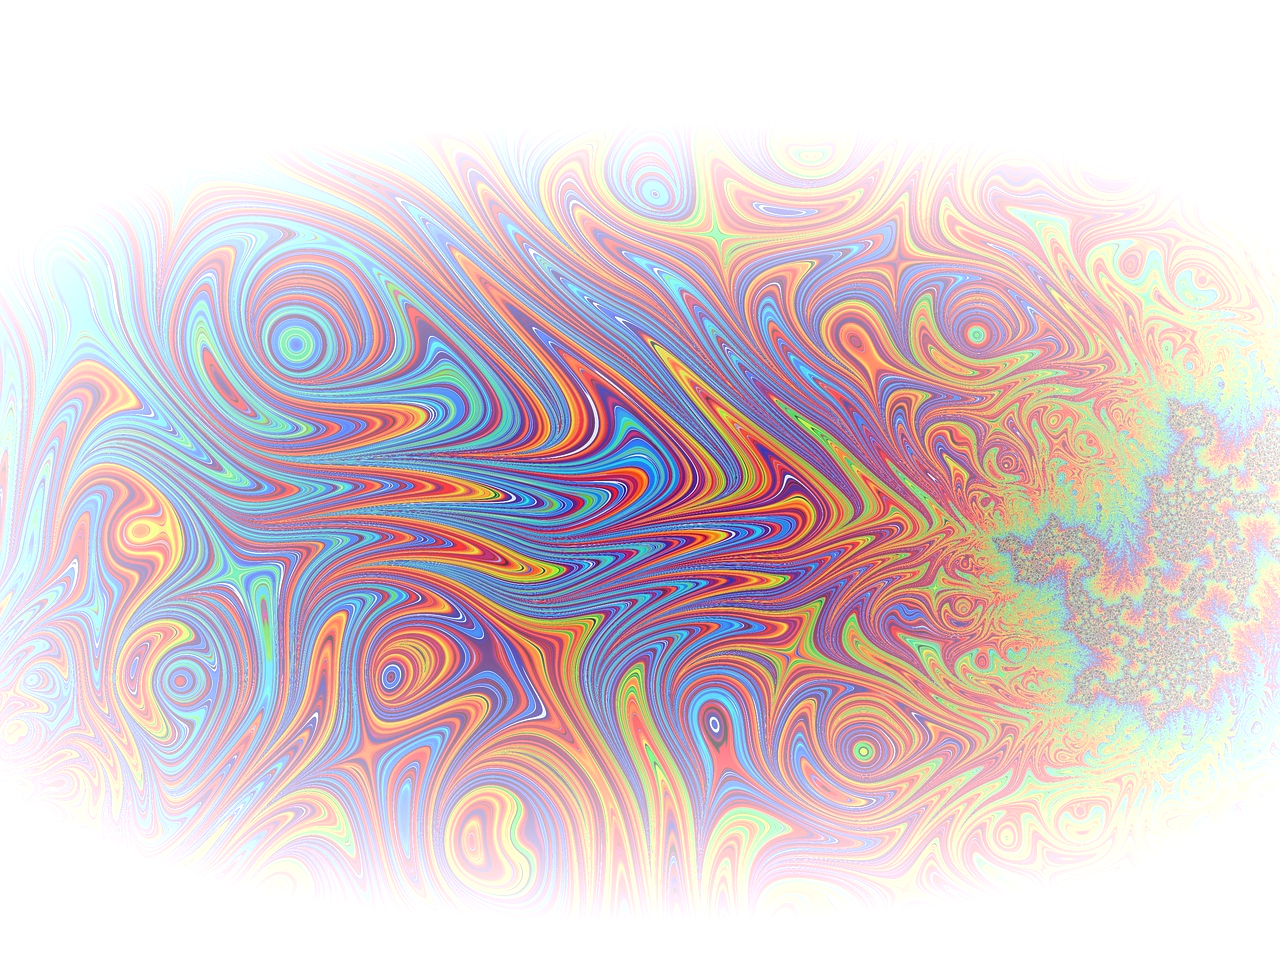
\includegraphics[width=\paperwidth,height=\paperheight]{fractal_2.jpg}%
}
\begin{frame}{... what Agda really sees}
	\smaller
	\vspace{20.2em}
	\remark{\textit{(Artistically Interpreted)}}
\end{frame}
}


{
\setbeamertemplate{background}{%
  \tikz[remember picture, overlay]
    \shade[top color=gray!05, bottom color=gray!95]
      (current page.north west) rectangle (current page.south east);%
}
\begin{frame}{... what you show the LLM}
\smaller
{\scriptsize
\begin{minipage}{1.\textwidth}
	\token{open}
	\token{ import}
	\token{ Relation}
	\token{.Binary}
	\token{.Pro}
	\token{pos}
	\token{itional}
	\token{Equality}
	\token{ using}
	\token{ (_}
	\token{≡}
	\token{_;}
	\token{ refl}
	\token{;}
	\token{ cong}
	\token{;}
	\token{ trans}
	\token{)<newline><newline>}
	\token{data}
	\token{ }
	\token{ℕ}
	\token{ :}
	\token{ Set}
	\token{ where}
	\token{<newline>}
	\token{  }
	\token{ zero}
	\token{ :}
	\token{ }
	\token{ℕ}
	\token{<newline>}
	\token{  }
	\token{ suc}
	\token{ }
	\token{ :}
	\token{ }
	\token{ℕ}
	\token{ →}
	\token{ }
	\token{ℕ}
	\token{<newline><newline>}
	\token{_}
	\token{+}
	\token{_}
	\token{ :}
	\token{ }
	\token{ℕ}
	\token{ →}
	\token{ }
	\token{ℕ}
	\token{ →}
	\token{ }
	\token{ℕ}
	\token{<newline>}
	\token{zero}
	\token{ +}
	\token{ n}
	\token{ =}
	\token{ n}
	\token{<newline>}
	\token{s}
	\token{uc}
	\token{ m}
	\token{ +}
	\token{ n}
	\token{ =}
	\token{ suc}
	\token{ (}
	\token{m}
	\token{ +}
	\token{ n}
	\token{)<newline><newline>}
	\token{+-}
	\token{comm}
	\token{ :}
	\token{ (}
	\token{m}
	\token{ n}
	\token{ :}
	\token{ }
	\token{ℕ}
	\token{)}
	\token{ →}
	\token{ m}
	\token{ +}
	\token{ n}
	\token{ }
	\token{≡}
	\token{ n}
	\token{ +}
	\token{ m}
	\token{<newline>}
	\token{+-}
	\token{comm}
	\token{ zero}
	\token{ zero}
	\token{ =}
	\token{ refl}
	\token{<newline>}
	\token{+-}
	\token{comm}
	\token{ zero}
	\token{ (}
	\token{s}
	\token{uc}
	\token{ n}
	\token{)}
	\token{ =}
	\token{ cong}
	\token{ suc}
	\token{ (+}
	\token{-}
	\token{comm}
	\token{ zero}
	\token{ n}
	\token{)<newline>}
	\token{+-}
	\token{comm}
	\token{ (}
	\token{s}
	\token{uc}
	\token{ m}
	\token{)}
	\token{ zero}
	\token{ =}
	\token{ cong}
	\token{ suc}
	\token{ (+}
	\token{-}
	\token{comm}
	\token{ m}
	\token{ zero}
	\token{)<newline>}
	\token{+-}
	\token{comm}
	\token{ (}
	\token{s}
	\token{uc}
	\token{ m}
	\token{)}
	\token{ (}
	\token{s}
	\token{uc}
	\token{ n}
	\token{)}
	\token{ =}
	\token{ cong}
	\token{ suc}
	\token{ (}
	\token{trans}
	\token{ (+}
	\token{-}
	\token{s}
	\token{uc}
	\token{ m}
	\token{ n}
	\token{)}
	\token{ (+}
	\token{-}
	\token{comm}
	\token{ (}
	\token{s}
	\token{uc}
	\token{ m}
	\token{)}
	\token{ n}
	\token{))<newline>}
	\token{  }
	\token{ where}
	\token{ +-}
	\token{s}
	\token{uc}
	\token{ :}
	\token{ }
	\token{∀}
	\token{ m}
	\token{ n}
	\token{ →}
	\token{ m}
	\token{ +}
	\token{ suc}
	\token{ n}
	\token{ }
	\token{≡}
	\token{ suc}
	\token{ (}
	\token{m}
	\token{ +}
	\token{ n}
	\token{)<newline>}
	\token{        }
	\token{ +-}
	\token{s}
	\token{uc}
	\token{ zero}
	\token{ n}
	\token{ =}
	\token{ refl}
	\token{<newline>}
	\token{        }
	\token{ +-}
	\token{s}
	\token{uc}
	\token{ (}
	\token{s}
	\token{uc}
	\token{ m}
	\token{)}
	\token{ n}
	\token{ =}
	\token{ cong}
	\token{ suc}
	\token{ (+}
	\token{-}
	\token{s}
	\token{uc}
	\token{ m}
	\token{ n}
	\token{)}
\end{minipage}
}

\vspace{-4.5em}
\remark{Where did all the colors go? \emoji{cloud}}%
\end{frame}
}

\begin{frame}{Doing things ``right''}
	\begin{center}
		
\includegraphics[width=0.65\pagewidth]{done_right.jpg}
	\end{center}

	\vfill
	\remark{\emoji{clown-face}}
\end{frame}

\begin{frame}{Doing things right}
	\smaller
	\textbf{Contributions:}
	\begin{itemize}[topsep=-0.25\baselineskip]
		\item \textit{Structured Machine Learning Data for Agda}.
		\item \textit{Learning to Represent (the Shapes of) Dependent Types.}
	\end{itemize}
\end{frame}


\begin{frame}{Data Extraction}
\smaller

\alt<16->{
	\visible<17->{
	\hspace{1.15cm}\begin{tikzpicture}[
			ast/.style={draw,gray,thick,outer sep=2pt,opacity=0.5},
			lab/.style={font=\large},
			ref/.style={->,dashed,gray,opacity=0.4,thick},
			var/.style={gray,opacity=0.8,execute at begin node={\strut(},execute at end node=)},
			t/.style={text height=1.5ex, text depth=.25ex, rectangle, outer sep=0pt},
			scale=1, transform shape]
		\tikzset{level 1/.style={level distance=22pt}, edge from parent/.append style={thick}}
		\Tree
		[.\node(t11) {•};
			[.\node{@};
				[.\node{@};
					\AgdaDatatype{≡}
					\AgdaBound{n}
				]
				[.\node{@};
					[.\node{@};
						\AgdaOperator{\AgdaFunction{+}}
						\AgdaBound{n}
					]
					\AgdaInductiveConstructor{zero}
				]
			]
		]
	\end{tikzpicture}}
}{%
\begin{minipage}{0.9\textwidth}
	\begin{code}%
	\uncover<-14,16->{\uncover<1,8->{\uncover<-4,8->{\uncover<-13,15->{%
	\>[0]\AgdaKeyword{open}\AgdaSpace{}%
	\AgdaKeyword{import}\AgdaSpace{}%
	\AgdaModule{Relation.Binary.PropositionalEquality}\AgdaSpace{}%
	\AgdaKeyword{using}\AgdaSpace{}%
	\AgdaSymbol{(}}\AgdaOperator{\AgdaDatatype{\AgdaUnderscore{}≡\AgdaUnderscore{}}}\uncover<-13,15->{\AgdaSymbol{;}}\AgdaSpace{}%
	\AgdaInductiveConstructor{refl}\uncover<-13,15->{\AgdaSymbol{;}}\AgdaSpace{}%
	\AgdaFunction{cong}\uncover<-13,15->{\AgdaSymbol{;}}\AgdaSpace{}%
	\AgdaFunction{trans}\uncover<-13,15->{\AgdaSymbol{)}\<%
	}}}}
	\end{code}
	
	\vspace{-1.25em}
	\begin{minipage}{.3\linewidth}
	\begin{code}%
	\uncover<-14,16->{\uncover<1,2,8->{\uncover<-4,8->{\uncover<-13,15->{%
	\>[0]%
	\AgdaKeyword{data}\AgdaSpace{}}%
	\AgdaDatatype{ℕ}\uncover<-13,15->{\AgdaSpace{}%
	\AgdaSymbol{:}\AgdaSpace{}%
	\AgdaPrimitive{Set}\AgdaSpace{}%
	\AgdaKeyword{where}\<%
	\\
	\>[0][@{}l@{\AgdaIndent{0}}]%
	\>[2]\AgdaInductiveConstructor{zero}%
	\>[8]\AgdaSymbol{:}\AgdaSpace{}%
	\AgdaDatatype{ℕ}\<%
	\\
	%
	\>[2]\AgdaInductiveConstructor{suc}%
	\>[8]\AgdaSymbol{:}\AgdaSpace{}%
	\AgdaDatatype{ℕ}\AgdaSpace{}%
	\AgdaSymbol{→}\AgdaSpace{}%
	\AgdaDatatype{ℕ}\<%
	}}}}
	\end{code}
	\end{minipage}
	
	\vspace{-1.25em}
	\begin{minipage}{.5\linewidth}
	\begin{code}%
	\>[0]\uncover<-14,16->{\uncover<1,3,5,8->{\AgdaOperator{\AgdaFunction{\AgdaUnderscore{}+\AgdaUnderscore{}}}}\AgdaSpace{}%
	\uncover<-13,15->{\uncover<1,3,8->{\AgdaSymbol{:}}\AgdaSpace{}%
	\uncover<1,3,6,8->{\AgdaDatatype{ℕ}\AgdaSpace{}%
	\AgdaSymbol{→}\AgdaSpace{}%
	\AgdaDatatype{ℕ}\AgdaSpace{}%
	\AgdaSymbol{→}\AgdaSpace{}%
	\AgdaDatatype{ℕ}}\<%
	\\
	\>[0]\uncover<1,3,7,8->{\AgdaInductiveConstructor{zero}%
	\>[7]\AgdaOperator{\AgdaFunction{+}}\AgdaSpace{}%
	\AgdaBound{n}\AgdaSpace{}%
	\AgdaSymbol{=}\AgdaSpace{}%
	\AgdaBound{n}\<%
	\\
	\>[0]\AgdaInductiveConstructor{suc}\AgdaSpace{}%
	\AgdaBound{m}%
	\>[7]\AgdaOperator{\AgdaFunction{+}}\AgdaSpace{}%
	\AgdaBound{n}\AgdaSpace{}%
	\AgdaSymbol{=}\AgdaSpace{}%
	\AgdaInductiveConstructor{suc}\AgdaSpace{}%
	\AgdaSymbol{(}\AgdaBound{m}\AgdaSpace{}%
	\AgdaOperator{\AgdaFunction{+}}\AgdaSpace{}%
	\AgdaBound{n}\AgdaSymbol{)}\<%
	}}}
	\end{code}
	\end{minipage}
	
	\vspace{-1.25em}
	\begin{code}%
	\uncover<1,4,8->{\uncover<-4,8->{%
	\>[0]\uncover<-14,16->{\AgdaFunction{+-comm}}\AgdaSpace{}%
	\uncover<-13,15->{\uncover<-14,16->{%
	\AgdaSymbol{:}\AgdaSpace{}%
	\AgdaSymbol{(}\AgdaBound{m}\AgdaSpace{}%
	\AgdaBound{n}\AgdaSpace{}%
	\AgdaSymbol{:}\AgdaSpace{}%
	\AgdaDatatype{ℕ}\AgdaSymbol{)}\AgdaSpace{}%
	\AgdaSymbol{→}\AgdaSpace{}%
	\AgdaBound{m}\AgdaSpace{}%
	\AgdaOperator{\AgdaFunction{+}}\AgdaSpace{}%
	\AgdaBound{n}\AgdaSpace{}%
	\AgdaOperator{\AgdaDatatype{≡}}\AgdaSpace{}%
	\AgdaBound{n}\AgdaSpace{}%
	\AgdaOperator{\AgdaFunction{+}\AgdaSpace{}%
	\AgdaBound{m}}\<%
	\\
	\>[0]\AgdaFunction{+-comm}\AgdaSpace{}%
	\AgdaInductiveConstructor{zero}%
	\>[16]\AgdaInductiveConstructor{zero}%
	\>[25]\AgdaSymbol{=}\AgdaSpace{}%
	\hole{9}{\AgdaInductiveConstructor{refl}}\<
	\\
	\>[0]\AgdaFunction{+-comm}\AgdaSpace{}%
	\AgdaInductiveConstructor{zero}%
	\>[16]\AgdaSymbol{(}\AgdaInductiveConstructor{suc}\AgdaSpace{}}%
	\AgdaBound{n}\uncover<-14,16->{\AgdaSymbol{)}%
	\>[25]\AgdaSymbol{=}\AgdaSpace{}%
	}}%
	\uncover<-13,16->{\AgdaFunction{cong}\AgdaSpace{}%
	\AgdaInductiveConstructor{suc}}\AgdaSpace{}%
	\hole{12-16}{%
	\AgdaSymbol{(}\AgdaFunction{+-comm}\AgdaSpace{}%
	\hole{11}{\AgdaInductiveConstructor{zero}}\AgdaSpace{}%
	\hole{10}{\AgdaBound{n}}\AgdaSymbol{)}}\<%
	\\
	\uncover<-13,16->{%
	\>[0]\AgdaFunction{+-comm}\AgdaSpace{}%
	\AgdaSymbol{(}\AgdaInductiveConstructor{suc}\AgdaSpace{}%
	\AgdaBound{m}\AgdaSymbol{)}%
	\>[16]\AgdaInductiveConstructor{zero}%
	\>[25]\AgdaSymbol{=}\AgdaSpace{}%
	\AgdaFunction{cong}\AgdaSpace{}%
	\AgdaInductiveConstructor{suc}\AgdaSpace{}%
	\AgdaSymbol{(}\AgdaFunction{+-comm}\AgdaSpace{}%
	\AgdaBound{m}\AgdaSpace{}%
	\AgdaInductiveConstructor{zero}\AgdaSymbol{)}\<%
	\\
	\>[0]\AgdaFunction{+-comm}\AgdaSpace{}%
	\AgdaSymbol{(}\AgdaInductiveConstructor{suc}\AgdaSpace{}%
	\AgdaBound{m}\AgdaSymbol{)}%
	\>[16]\AgdaSymbol{(}\AgdaInductiveConstructor{suc}\AgdaSpace{}%
	\AgdaBound{n}\AgdaSymbol{)}%
	\>[25]\AgdaSymbol{=}\AgdaSpace{}%
	\AgdaFunction{cong}\AgdaSpace{}%
	\AgdaInductiveConstructor{suc}\AgdaSpace{}%
	\AgdaSymbol{(}\AgdaFunction{trans}\AgdaSpace{}%
	\AgdaSymbol{(}\AgdaFunction{+-suc}\AgdaSpace{}%
	\AgdaBound{m}\AgdaSpace{}%
	\AgdaBound{n}\AgdaSymbol{)}\AgdaSpace{}%
	\AgdaSymbol{(}\AgdaFunction{+-comm}\AgdaSpace{}%
	\AgdaSymbol{(}\AgdaInductiveConstructor{suc}\AgdaSpace{}%
	\AgdaBound{m}\AgdaSymbol{)}\AgdaSpace{}%
	\AgdaBound{n}\AgdaSymbol{))}\<%
	\\
	\>[0][@{}l@{\AgdaIndent{0}}]%
	\>[2]\AgdaKeyword{where}%
	\>[73I]\AgdaFunction{+-suc}\AgdaSpace{}%
	\AgdaSymbol{:}\AgdaSpace{}%
	\AgdaSymbol{∀}\AgdaSpace{}%
	\AgdaBound{m}\AgdaSpace{}%
	\AgdaBound{n}\AgdaSpace{}%
	\AgdaSymbol{→}\AgdaSpace{}%
	\AgdaBound{m}\AgdaSpace{}%
	\AgdaOperator{\AgdaFunction{+}}\AgdaSpace{}%
	\AgdaInductiveConstructor{suc}\AgdaSpace{}%
	\AgdaBound{n}\AgdaSpace{}%
	\AgdaOperator{\AgdaDatatype{≡}}\AgdaSpace{}%
	\AgdaInductiveConstructor{suc}\AgdaSpace{}%
	\AgdaSymbol{(}\AgdaBound{m}\AgdaSpace{}%
	\AgdaOperator{\AgdaFunction{+}}\AgdaSpace{}%
	\AgdaBound{n}\AgdaSymbol{)}\<%
	\\
	\>[.][@{}l@{}]\<[73I]%
	\>[8]\AgdaFunction{+-suc}\AgdaSpace{}%
	\AgdaInductiveConstructor{zero}%
	\>[23]\AgdaBound{n}\AgdaSpace{}%
	\AgdaSymbol{=}\AgdaSpace{}%
	\AgdaInductiveConstructor{refl}\<%
	\\
	\>[8]\AgdaFunction{+-suc}\AgdaSpace{}%
	\AgdaSymbol{(}\AgdaInductiveConstructor{suc}\AgdaSpace{}%
	\AgdaBound{m}\AgdaSymbol{)}%
	\>[23]\AgdaBound{n}\AgdaSpace{}%
	\AgdaSymbol{=}\AgdaSpace{}%
	\AgdaFunction{cong}\AgdaSpace{}%
	\AgdaInductiveConstructor{suc}\AgdaSpace{}%
	\AgdaSymbol{(}\AgdaFunction{+-suc}\AgdaSpace{}%
	\AgdaBound{m}\AgdaSpace{}%
	\AgdaBound{n}\AgdaSymbol{)}\<%
	}}}
	\end{code}
\end{minipage}
}\vfill

\begin{tikzpicture}[remember picture, overlay, shift={(current page.south west)}, shift={(1cm, 1cm)}]
	\visible<2>{
		\draw[rounded corners, thick, red] (0.7cm, 4.9cm) rectangle (3.6cm, 5.9cm);
    }
	\visible<3,5-7>{
		\draw[rounded corners, thick, red] (0.7cm, 3.6cm) rectangle (3.6cm, 4.7cm);
	}
	\visible<4>{
		\draw[rounded corners, thick, red] (0.7cm, 0.8cm) rectangle (9.5cm, 3.5cm);
	}

	\node[anchor=west, text width=7.5cm, text depth=0.25ex, text height=1.5ex] at (7.5cm, 5cm) {\alt<8->{%
		\alt<16->{%
			\begin{itemize}
			\item[3.] Each term \& type is recorded as both:\vspace{-0.3em}
				\begin{itemize}
					\item a pretty string
					\visible<17->{\item the underlying AST}
				\end{itemize}
			\end{itemize}
			
		}{%
			\begin{itemize}
				\item[2.] We go through all \textbf{subterms}.\\
				\visible<13-15>{For each subterm, we record:\vspace{-0.3em}
				\begin{itemize}
					\item its type \light{(/the goal)}
					\visible<14->{\item its scope}
					\visible<15->{\item its context}
				\end{itemize}
			}
			\end{itemize}
		}
    }{%
		\begin{itemize}
			\item[1.] We go through \textbf{all definitions}.\\
			\visible<5->{For each definition, we record:\vspace{-0.3em}
			\begin{itemize}
				\item its name
				\visible<6->{\item its type}
				\visible<7->{\item its term \light{(/proof)}}
			\end{itemize}
		}
		\end{itemize}
	}};

	\visible<13, 16->{
		\node[anchor=west, text width=7.5cm, text depth=0.25ex, text height=1.5ex] at (0.7cm, -0.2cm) {\texttt{\textcolor{red}{goal: n ≡ (n + zero)}}};
	}
\end{tikzpicture}
\end{frame}

\begin{frame}{Data: TL;DR}
	\smaller
	\textbf{Niceties}:
	\begin{itemize}
		\item among first ML datasets for Agda
		\item subterm iteration $\implies$ type-checked data augmentation for free
		\item extraction explicitly preserving type-structure
	\end{itemize}\vfill
	
	\visible<2->{
	\textbf{Numerical}\textsuperscript{1}:
	\begin{itemize}
		\item \eqmakebox[num][l]{800} modules
		\item \eqmakebox[n2][l]{\eqmakebox[num][l]{11.751} definitions}
		\item \eqmakebox[n2][l]{\eqmakebox[num][l]{67.255} ``holes'' \light{read: data points}}
	\end{itemize}\vfill

	\hrule\vspace{0.3em}
	\light{\smaller 1: passing extracts from \texttt{agda-stdlib} 1.7.2}
	}
\end{frame}

\begin{frame}{Representation Learning \alt<6->{2}{1}\\
\smaller\light{\hphantom{xx} \alt<7->{Amending self-attention}{\alt<6->{How to represent it?}{What's to represent?}}}}
	\smaller
	\alt<6>{
		\textbf{Candidate Architectures}:
		\begin{itemize}
			\item \eqmakebox[architecture][l]{\st{LLMs}} \light{-\,- \textit{just no}}
			\item \eqmakebox[architecture][l]{\st{GNNs}} \light{-\,- \textit{too generic, oversmoothing}}
			\item \eqmakebox[architecture][l]{\st{Tree (R)NNs}} \light{-\,- \textit{too slow, generally under-performing}}
			\item \eqmakebox[architecture][l]{Full Attention [\light{?}]} \light{-\,- \textit{no structural biases}}\\
			\eqmakebox[architecture][l]{} \light{-\,- \textit{${\left(\sum_t^T n(t)\right)}^2$ scaling}}\\
		\end{itemize}\vfill
	}{
	\vspace{-4.5em}
	\centering\begin{tikzpicture}[
			ast/.style={draw,gray,thick,outer sep=2pt,opacity=0.5},
			lab/.style={font=\large},
			ref/.style={->,dashed,gray,opacity=0.45,thick, shorten >=4pt},
			prim/.style={},
			var/.style={gray,execute at begin node={\strut(},execute at end node=)},
			var2/.style={gray,execute at begin node={\strut(},execute at end node=)},
			var3/.style={gray},
			t/.style={text height=1.5ex, text depth=.25ex, rectangle, outer sep=0pt},
			scale=0.65, transform shape]
		\only<2>{\tikzset{prim/.style={draw=red}}}
		\only<3>{\tikzset{var/.append style={draw=red}}}
		\only<4>{\tikzset{var2/.append style={draw=red}}}
		\only<5>{\tikzset{var3/.append style={draw=red}}}
		\tikzset{level 1/.style={level distance=22pt}, edge from parent/.append style={thick}}
		\begin{scope}[xshift=0cm]
		\Tree
		[.\node(t11) {•};
				\node[prim] (t12) {\AgdaPrimitive{Set}};
		]
		\alt<3>{
			\node[ast,draw=red,fit=(t11)(t12)](nat) {};
		}{
			\node[ast,fit=(t11)(t12)](nat) {};
		}
		\node[lab,xshift=5.5pt,yshift=4pt]() at(nat.north west) {\AgdaDatatype{ℕ}};
		\begin{scope}[xshift=3.75cm,yshift=-1.5cm]
		\Tree
		[.\node (t21) {•};
			[.\node[prim]{$\to$};
				\node[var] (plus-l) {\AgdaDatatype{ℕ}};
				[.\node[prim]{$\to$};
					\node[var] (plus-r) {\AgdaDatatype{ℕ}};
					\node[var] (plus-out) {\AgdaDatatype{ℕ}};
				]
			]
		]
		\alt<4>{
			\node[ast,draw=red,fit=(t21)(plus-l)(plus-out)] (+) {};
		}{
			\node[ast,fit=(t21)(plus-l)(plus-out)] (+) {};
		}
		\node[lab,xshift=4.5pt,yshift=4pt]() at(+.north west) {\AgdaFunction{+}};
		\begin{scope}[xshift=6.5cm,yshift=3.2cm]\Tree
		[.\node (t31) {•};
			[.\node[prim]{$\Pi$};
				\node[var,var3] (m-def) {$\AgdaBound{m}:\AgdaPrimitive{ℕ}$};
				[.\node[prim]{$\Pi$};
					\node[var,var3] (n-def) {$\AgdaBound{n}:\AgdaPrimitive{ℕ}$};
					[.\node[prim]{@};
						[.\node[prim]{@};
							\node[prim]{\AgdaPrimitive{≡}};
							[.\node[prim]{@};
								[.\node[prim]{@};
									\node[var2] (+-ref-1) {\AgdaFunction{+}};
									\node[var3] (m-ref-1) {\AgdaBound{m}};
								]
								\node[var3] (n-ref-1) {\AgdaBound{n}};
							]
						]
						[.\node[prim]{@};
							[.\node[prim]{@};
								\node[var2] (+-ref-2) {\AgdaFunction{+}};
								\node[var3] (n-ref-2) {\AgdaBound{n}};
							]
							\node[var3] (m-ref-2) {\AgdaBound{m}};
						]
					]
				]
			]
		]
		\node[ast,fit=(t31)(m-def)(+-ref-1)(m-ref-2)] (comm) {};
		\node[lab,xshift=19pt,yshift=4pt]() at(comm.north west) {\AgdaFunction{+-comm}};
		\end{scope}\end{scope}\end{scope}
		\visible<3-6,9,13>{
			\draw[ref,var] (plus-l) -- (nat);
			\draw[ref,var] (plus-r) -- (nat);
			\draw[ref,var] (plus-out) -- (nat);
		}
		\visible<3-6,10,13>{
			\draw[ref,var] (m-def) -- (nat);
			\draw[ref,var] (n-def) -- (nat);
		}
		\visible<4-6,10,13>{
			\draw[ref,var2] (+-ref-1) -- (+);
			\draw[ref,var2] (+-ref-2) -- (+);
		}
		\visible<5-6,12->{
			\draw[ref,var3] (m-ref-1) -- (m-def);
			\draw[ref,var3] (m-ref-2) -- (m-def);
			\draw[ref,var3] (n-ref-1) -- (n-def);
			\draw[ref,var3] (n-ref-2) -- (n-def);
		}
	\end{tikzpicture}
	
	\visible<-6>{
	\begin{tikzpicture}[remember picture, overlay, shift={(current page.south west)}]
		\node[anchor=west, text width=7.5cm, text depth=0.25ex, text height=1.5ex] at (0.75cm, 2cm) {
			\alt<2->{A sequence of ASTs, where nodes are:}{A sequence of ASTs}
				\begin{itemize}
					\visible<2->{\item TT primitives}
					\visible<3->{\item references to (other) lemmas (inter-AST)}
					\visible<5->{\item references to bound variables (intra-AST)}
				\end{itemize}
		};
	\end{tikzpicture}
	}
	
	\visible<7->{
		\visible<8-10>{
			\begin{tikzpicture}[remember picture, overlay, shift={(current page.south west)}]
				\draw[red, thick] plot [smooth cycle, tension=0.9] coordinates {(2.9,5.5) (4, 5.5) (4, 6.9) (2.9, 6.9)};
				\draw[red, thick] plot [smooth cycle, tension=0.9] coordinates {(2.88,5.57) (4.05, 5.48) (3.99, 6.9) (2.9, 6.95)};
				\node (1) at (3.9, 6.75) {\Large\textcolor{red}{0}};
				\visible<9->{
					\draw[red, thick] plot [smooth cycle, tension=1] coordinates {(5, 3.1) (7, 3.1) (7,5.9) (5, 5.9)};
					\draw[red, thick] plot [smooth cycle, tension=1] coordinates {(4.95, 3.1) (6.95, 3.05) (7.05,5.9) (5, 5.85)};
					\node (2) at (6.6, 5.85) {\Large\textcolor{red}{1}};
				}
				\visible<10->{
					\draw[red, thick] plot [smooth cycle, tension=0.8] coordinates {(8.5, 2.8) (13.5, 2.8) (13.2, 7.5) (8.5, 7.8)};
					\draw[red, thick] plot [smooth cycle, tension=0.8] coordinates {(8.55, 2.75) (13.45, 2.85) (13.2, 7.5) (8.5, 7.85)};
					\node (3) at (12, 7.85) {\Large\textcolor{red}{2}};
				}
			\end{tikzpicture}
		}
		\begin{tikzpicture}[remember picture, overlay, shift={(current page.south west)}]
			\node[anchor=west, text width=10.5cm, text depth=0.25ex, text height=1.5ex] at (0.75cm, 2.3cm) {
				\alt<13->{Representations informed by \textbf{type shapes} alone:
					\begin{itemize}
						\item invariance to $\alpha$-renaming, scope permutations, syntactic distractions, etc.
						\item \light{\dots but a few things get lost in translation}
					\end{itemize}
				}{
				\begin{itemize}
					\item \eqmakebox[improvement][l]{Treewise \underline{Linear} (Taylor Series) Attention} \light{-\,- $\#T \times\mathop{\mathrm{max}}_t^T n(t)$ scaling}\\
					\visible<8->{\item \eqmakebox[improvement][l]{Dependency-Level Batching} \light{-\,- explicit scope referencing}}
					\visible<11->{\item \eqmakebox[improvement][l]{Relative Tree-PE} \light{-\,- proper inductive biases}\\
					\visible<12->{\eqmakebox[improvement][l]{} \light {-\,- \& dynamic variable indexing}}
					}
				\end{itemize}
				}
			};
		\end{tikzpicture}
	}
}
\end{frame}

\begin{frame}{Experimental Setup}
	\smaller
	\textbf{Premise Selection}\\
	Contextually rank scope entries by their relevance to the current goal.\vfill
	
		\textbf{\agdaQuill} \emoji{feather}\\
	Tiny PoC model (\light{6L $\times$ 8H $\times$ 256D; 1 mil. params; 25MB@FP32}) trained for $\sim$8h on a V100\vfill
	
	\textbf{Data}
	\begin{itemize}
		\item train on random holes from 85\% of \texttt{agda-stdlib} (ignoring size outliers)
		\item eval on unseen proofs from:\vspace{-0.15em}
		\begin{itemize}
			\item remaining 15\% (split between \textsc{id} and \textsc{ood} on the basis of size)
			\item \texttt{Unimath} \& \texttt{TypeTopology} (distant domains)
		\end{itemize}
	\end{itemize}
\end{frame}

\begin{frame}{... but does it work?}
	\smaller
	\alt<2->{
		\alt<3->{
			\vspace{2.5em}
		\textbf{Findings, TL;DR}
		\begin{itemize}
			\item high performance despite limited expressivity \& no term exposition
			\item structure preservation outweights architectural optimizations
			\item baseline encoder collapses
		\end{itemize}
		}{
		\textbf{Less obscure visualization}
	
		\begin{center}
			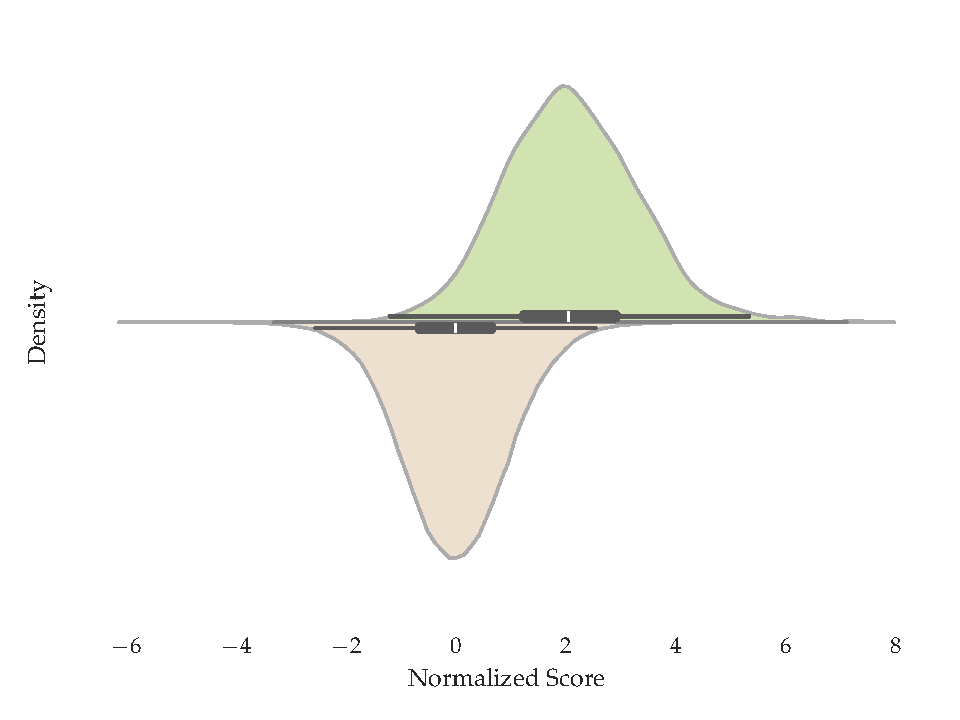
\includegraphics[width=0.65\textwidth, trim={0 3em 0 4em}, clip]{violin.pdf}
		\end{center}
		\light{Empirical distribution of selection scores of relevant (green) vs irrelevant (red) lemmas (\stdlib{}:\textsc{id}).}
		}
	}{
	\vspace{2.5em}
	\textbf{Mandatory table with numbers}
	\begin{center}\vspace{-0.5em}
	\newcolumntype{C}{>{\centering\arraybackslash}X}
	\newcolumntype{L}{>{\raggedright\arraybackslash}X}
	\newcolumntype{R}{>{\raggedleft\arraybackslash}X}
	\begin{tabularx}{0.8\textwidth}{
		@{}l@{\quad}L@{~/~}R@{\quad}R@{~/~}L@{\quad}R@{~/~}L@{\quad}R@{~/~}L@{}
	}
	& \multicolumn{8}{c}{Average / R-Precision}\\
	\cmidrule{2-9}
	\multicolumn{1}{@{}l}{\textsc{Model}}
	& \multicolumn{2}{@{\quad}C@{\quad}}{\stdlib{}:\textsc{id}}
	& \multicolumn{2}{C@{\quad}}{\stdlib{}:\textsc{ood}}
	& \multicolumn{2}{@{\quad}C@{\quad}}{\unimath}
	& \multicolumn{2}{@{\quad}C@{\quad}}{\typetopo}\\
	\toprule
	~\agdaQuill 	&
		\bfstat{50.2}{0.5} & \bfstat{40.3}{0.4} & \bfstat{38.7}{0.7} & \bfstat{31.1}{0.9} & \bfstat{27.0}{0.4} & \bfstat{17.4}{0.3} & \bfstat{22.5}{0.3} & \bfstat{15.4}{0.5} \\
		\multicolumn{1}{c}{\vdots}\\
		~Transformer Baseline\textsuperscript{1} & \bstat{10.9}{0.4} & \sstat{3.7}{0.2} & \sstat{8.5}{0.2	} & \sstat{4.5}{0.1} & \sstat{9.4}{0.3} & \sstat{3.9}{0.1} & \sstat{5.8}{0.0} & \sstat{0.9}{0.0} \\
	\bottomrule	
	\end{tabularx}
	\end{center}\vfill
	
	\vspace{2.5em}
	\hrule
	\vspace{0.3em}
	\smaller 1: \light{no Tree-PE, no variable indexing resolution, no Taylor expansion in linear attention}
	}
\end{frame}

\begin{frame}{Suggested takehome messages}
	\smaller
	\vspace{3em}
	\begin{itemize}
		\item[\emoji{earth-africa}] the earth is not flat, proofs are not strings, LLMs are not the (only) answer
		\item[\emoji{key}] back-and-forth compiler integration is the key to better architectures
	\end{itemize}\vfill
	
	\hfill Thank you\vfill	
	
	\begin{itemize}
		\item \eqmakebox[names][l]{\textsc{Paper}}  -- \href{https://openreview.net/forum?id=e397soEZh8}{openreview.net/forum?id=e397soEZh8}\\
		\light{\textit{Published manuscript \& reviews.}}
		\item \eqmakebox[names][l]{\textsc{Agda2Train}} -- \href{https://github.com/omelkonian/agda2train}{github.com/omelkonian/agda2train}\\
		\light{\textit{Data extraction as an Agda \textit{compilation backend} (in Haskell).}}
		\item \eqmakebox[names][l]{\textsc{Agda-Quill}} -- \href{https://github.com/konstantinosKokos/quill}{github.com/konstantinoskokos/quill}\\
		\light{\textit{ML model; ML-facing Python interface for dataset reading \& processing.}}
	\end{itemize}\vfill
\end{frame}

\begin{frame}[plain]
	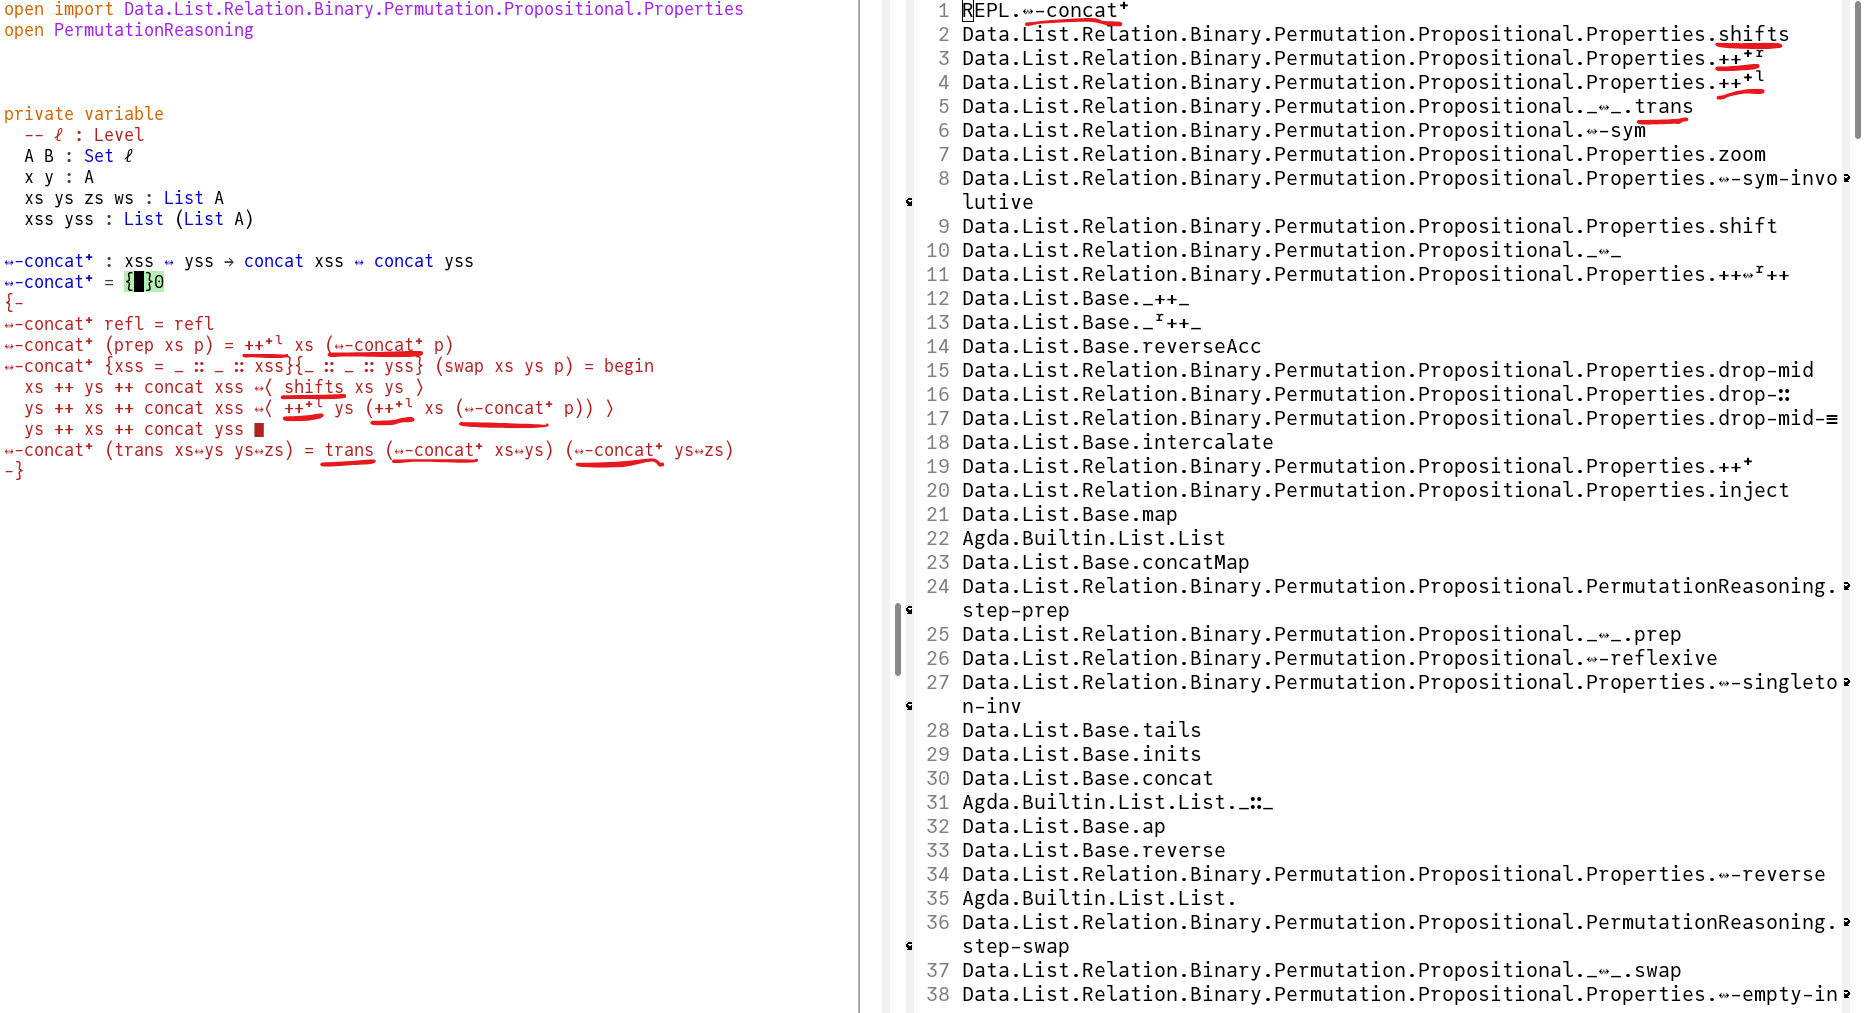
\includegraphics[width=\textwidth]{interface.png}
\end{frame}

\end{document}
